\subsection{Anarchic Model}

To justify this semantics capture all the possible abstract executions under certain consistency model,
we introduce \emph{anarchic model}.
Then by \cref{thm:consistency-intersect-anarchic},
the operational semantics captures all possible behaviours of a program \( \prog \) under certain consistency model.


\begin{definition}[Anarchic Model]
\label{def:anarchic-model}
The anarchic resolution policy $\RP_{\anarchic}$ is defined as 
$\RP_{\anarchic}(\_, \_) = \Snapshots$. The \emph{anarchic consistency model} is 
specified axiomatically by the pair $\anarchicCM = (\RP_{\anarchic}, \emptyset)$.
\end{definition}

Under the anarchic model, the initial snapshot of a transaction \( \txid \) is non-deterministic 
and does not depend on its observable transactions \( \T \).
When committing, the transaction \( \txid \) is always allowed to do so no matter the state of visibility relation.
Suppose a client $\cl$ has the transactional code below:
\[
\begin{session}
\ptrans{\pderef{\pvar{a}}{\ke}; \\
\pifs{\pvar{a} = \val_{1}} \pmutate{\ke'}{\val_1} \pife}
\end{session}
\]
%If the program is executed under a consistency model that adopts the last write 
%wins resolution policy $\RP_{\LWW}$, and with no additional axioms. 
%Then the behaviour of $\prog$ is completely deterministic (up-to the choice of transaction identifiers), 
%and the execution of $\prog$ terminates in a state corresponding to the abstract execution below: 

%\begin{center}
%\begin{tikzpicture}[scale=0.85, every node/.style={transform shape}]

%\node(t0rx) at (-1,2) {$(\otR, \ke, \val_0)$}; 
%%\path (t0wx.south) + (0,-0.2) node[anchor=north] (t0wy) {$(\otW, \ke_2, \val'_0)$};

%\begin{pgfonlayer}{background}
%\node[background, fit=(t0rx)]  {};

%\path(t0.west) node[anchor=east] (t0lbl) {$\txid_{\cl}^{\_}$};
%%\path(t1.north) node[anchor=south] (t1lbl) {$\txid_1$};
%%\path(t2.south) node[anchor=north] (t2lbl) {$\txid_2$};

%%\path[->]
%%(t0.north) edge[bend left=70] node[above, yshift=7pt, xshift=-1pt, pos=0.3] {$\RF(\ke_2), \VO(\ke_1)$} (t1.west)
%%(t0.south) edge[bend right=70] node[below, yshift=-8pt, xshift=-1pt, pos=0.3] {$\RF(\ke_1), \VO(\ke_2)$} (t2.west)
%%([xshift=-8pt]t2.north) edge[bend left=40] node[left] {$\AD(\ke_1)$} ([xshift=-8pt]t1.south) 
%%([xshift=8pt]t1.south) edge[bend left=40] node[right] {$\AD(\ke_2)$} ([xshift=8pt]t2.north);
%\end{pgfonlayer}
%\end{tikzpicture}
%\end{center}

Let consider executing the transaction under initial state with all keys set to the same initial value \( \val_0 \).
Under $\anarchicCM$, because the snapshot is chosen non-deterministically, 
the transaction might start with an initial snapshot where all keys have the value \( \val_1 \),
which are not necessary equal to \( \val_0 \).
Since there is no constraint on the visibility relation,
such transaction is always allowed to commit.
Consequently, the abstract execution after is the following: 
\begin{center}
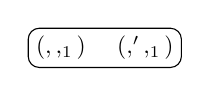
\begin{tikzpicture}[scale=0.85, every node/.style={transform shape}]

\node[rounded corners,draw](t0rx) {$(\otR, \ke, \val_1)$ \quad $(\otW, \ke', \val_1)$}; 

\end{tikzpicture}
\end{center}

It is important to note, however, that the set of abstract executions generated by $\prog$ 
is still bound to the structure of the program.
For example, executing $\prog$ under the anarchic execution model will never lead to 
an abstract execution with multiple transactions, 
or to an abstract execution where a transaction writes a key other than $\ke'$ is written.

The \cref{def:axiom-to-cm} defines all the possible abstract executions 
induced by a axiomatic specification $(\RP, \Ax)$.

\begin{definition}[Programs under axiomatic specification]
\label{def:axiom-to-cm}
\label{def:axiom-to-prog}
The semantics of a program $\prog$ under a consistency model with axiomatic specification 
$(\RP, \Ax)$ is given by 
\[
\interpr{\prog}_{(\RP, \Ax)} = \{ \aexec \mid (\aexec_{0}, \thdenv_{0}, \prog) \toA{\_}_{(\RP, \Ax)}^{\ast} (\aexec, \_, \prog_{f}) \}
\]
where $\thdenv_{0} = \lambda \cl \in \dom(\prog).\lambda \vx.0$ and $\prog_{f} = \lambda \cl \in \dom(\prog).\pskip$.
\end{definition}

We define the set of all the possible behaviours of a program $\prog$ to be $\interpr{\prog}_{\anarchic}$. 
One may argue that the axiomatic specification $\anarchicCM$ does not truly represent an anarchic consistency model. 
Consider the following code:
\[
\begin{session}
\ptrans{
\pderef{\pvar{a}}{\ke}; \\
\pderef{\pvar{b}}{\ke};\\
\pifs{\pvar{a} != \pvar{b}} \pmutate{\ke'}{\val_1} \pife}
\end{session}
\]
Under a even weaker anarchic consistency model, 
it would be possible for program $\prog'$ to write the value $\val_1$ for key $\ke'$. 
However, this never happens if $\prog'$ is executed under our $\anarchicCM$.
Because we embedded into abstract execution the assumption that 
transactions only read at most one value for each key.

We can weaken the anarchic behaviours further by lifting this limitation 
and still retain the validity of all the results contained in this report.
%However, doing so would require to work with mathematical structures that are far more complex than 
%abstract executions, and we preferred to avoid this issue. 
However, the constraint that an object is never read twice in transactions is enforced by atomic visibility, 
so it is unnecessary to lift such limitation of our $\anarchicCM$.
%When a client first requests to fetch the value of some key $\ke$ within a transaction, a local copy of the value fetched is 
%saved on the client (typically in an object containing the meta-data of the transaction); 
%if a request to read the same key is performed again within the same client, the local 
%copy of the value previously fetched for that key is returned, instead of issuing a second 
%read request to the kv-store.

The set of all possible behaviours exhibited by a program $\prog$ under a consistency model $(\RP, \Ax)$ 
can be defined by intersecting the set of executions that $\prog$ exhibits under the anarchic consistency model,
with the set of all executions allowed by the axiomatic specification $(\RP, \Ax)$ (\cref{thm:consistency-intersect-anarchic}).

\begin{theorem}
\label{thm:consistency-intersect-anarchic}
For any program $\prog$ and axiomatic specification $(\RP, \Ax)$:
\[
\interpr{\prog}_{(\RP, \Ax)} = \interpr{\prog}_{\anarchic} \cap \CMa(\RP, \Ax)
\]
\end{theorem}
\begin{proof}
    It is easy to see \( \interpr{\prog}_{(\RP, \Ax)} \subseteq \CMa(\RP, \Ax) \) by \cref{def:axiom-to-cm} 
    so \( \interpr{\prog}_{(\RP, \Ax)} \subseteq \interpr{\prog}_{\anarchic} \cap \CMa(\RP, \Ax) \).
    For another way, by \cref{prop:aexec-semantics-mono}, 
    we know \( \interpr{\prog}_{\anarchic} \subseteq \interpr{\prog}_{(\RP, \Ax)} \).
    Then, by the definition of \( \interpr{\prog}_{\stub} \), it follows
    \( \interpr{\prog}_{\anarchic} \cap \CMa(\RP, \Ax) \subseteq \interpr{\prog}_{(\RP, \Ax)} \).
\end{proof}


\begin{proposition}[Monotonic axiomatic specifications]
\label{prop:aexec-semantics-mono}
Let define \( (\RP_1, \Ax_1) \sqsubseteq (\RP_2, \Ax_2) \) as the following:
\[
    \fora{\aexec,\T} \RP_2(\aexec,\T) \subseteq \RP_1(\aexec,\T)
\]
and,
\[
    \fora{\aexec} \bigcup\limits_{\A_1 \in \Ax_1}\A_1(\aexec) \subseteq \bigcup\limits_{\A_2 \in \Ax_2}\A_2(\aexec)
\]
then
\[ \interpr{\prog}_{(\RP, \Ax)} \subseteq \interpr{\prog}_{\anarchic} \]
\end{proposition}
\begin{proof}
    Since \( \anarchic \sqsubseteq (\RP, \Ax) \),
    We prove stronger result that for \( (\RP_1, \Ax_1) \sqsubseteq  (\RP_2, \Ax_2)\),
    the following  hold:
    \[
        \begin{array}{@{}l@{}}
            \fora{\cl, \aexec, \aexec', \prog, \prog', \stk, \stk'} 
            \cl \vdash ( \aexec, \stk ), \prog \toA{\stub}_{(\RP_1, \Ax_1)} ( \aexec', \stk' ), \prog' 
            \implies \cl \vdash ( \aexec, \stk ), \prog \toA{\stub}_{(\RP_2, \Ax_2)} ( \aexec', \stk' ), \prog' \\
        \end{array}
    \]
    We prove it by induction on the derivations.
    The only interesting case is the \rl{PCommit} rule.
    Given an initial runtime abstract execution \( \aexec \),
    a set of observable transactions \( \T \),
    a new transaction identifier \( \txid \),
    by the \rl{ACommit} rule, it is sufficient to prove, 
    first, all the snapshot under the stronger consistency model is also a valid snapshot under the weaker one:
    \begin{equation}
        \label{equ:obs-state-included}
        \fora{\aexec,\T} \RP_2(\aexec,\T) \subseteq  \RP_1(\aexec,\T)
    \end{equation}
    and second if it is valid  to commit a new transition with the observable set \( \T \) under stronger consistency model,
    it is able to do so under weaker consistency model:
    \begin{equation}
        \label{equ:consis-both-exist}
        \bigcup\limits_{\A_1 \in \Ax_1}\A_1(\aexec')^{-1}(\txid) \subseteq \bigcup\limits_{\A_2 \in \Ax_2}\A_2(\aexec')^{-1}(\txid)
    \end{equation}
    The \cref{equ:obs-state-included,equ:consis-both-exist} can be proven by \( (\RP_1, \Ax_1) \sqsubseteq  (\RP_2, \Ax_2) \).

    \caseB{\rl{PAssign}, \rl{PAssume}, \rl{PChoice}, \rl{PLoop}, \rl{PSeqSkipS}, \rl{PPar}, \rl{PWait}}
    These base cases do not depend on the consistency model, so they trivial hold because of the hypothesis.
    \caseI{\rl{PSeq}}
    It is proved directly by applying the \ih
\end{proof}
